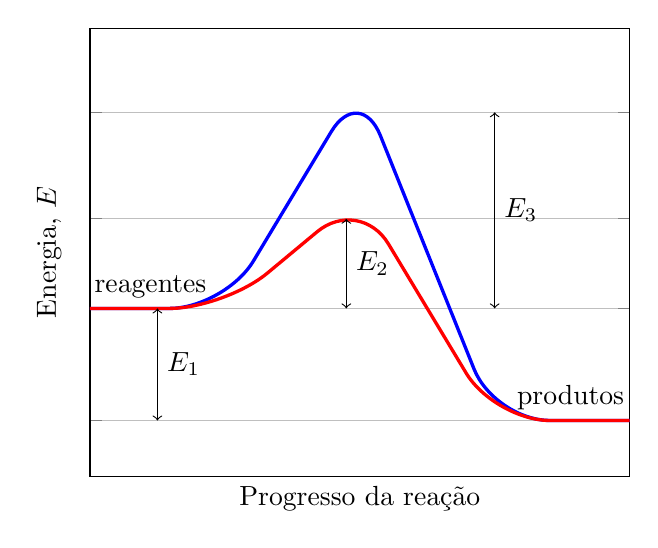
\begin{tikzpicture}
    \begin{axis}
        [
            ylabel = {Energia, $E$},
            xlabel = {Progresso da reação},
            xmin =  0.0, xmax = 4,
            ymin = -0.5, ymax = 3.5,
            xtick = \empty,
            ytick = {0, 1, 1.8, 2.75},
            yticklabels = {},
            grid  = major,
        ]
    \draw [draw=blue, very thick, rounded corners=2em]
        (axis cs: 0.0, 1.0) -- 
        (axis cs: 1.0, 1.0) -- 
        (axis cs: 2.0, 3.0) -- 
        (axis cs: 3.0, 0.0) --
        (axis cs: 4.0, 0.0);
    \draw [draw=red, very thick, rounded corners=2em]
        (axis cs: 0.0, 1.0) -- node [above] {reagentes \,}
        (axis cs: 1.0, 1.0) -- 
        (axis cs: 2.0, 2.0) -- 
        (axis cs: 3.0, 0.0) -- node [above] {\; produtos}
        (axis cs: 4.0, 0.0);
    \draw [draw=black, <->]
        (axis cs: 0.5, 0) -- node [right] {$E_1$}
        (axis cs: 0.5, 1);
    \draw [draw=black, <->]
        (axis cs: 1.9, 1) -- node [right] {$E_2$}
        (axis cs: 1.9, 1.8);
    \draw [draw=black, <->]
        (axis cs: 3.0, 1) -- node [right] {$E_3$}
        (axis cs: 3.0, 2.75);
     \end{axis}
 \end{tikzpicture}
